\chapter{Project Management}
\section{Terms}
Here follows a description of terms that are useful to understand how the project management functioned. 

\begin{description}
\item[Scrum] \label{def:scrum}is an popular agile software development methodology. This means that the work is done in increments called sprints, and daily meetings are held to update the rest of the team on progress and problems. The scrum process also has roles for team members, in particular a team member called scrum master who handles contact between the development team and people outside the team.

\item[Sprint] \label{def:sprint} is a period in which work is planned and done. It has a duration of one week. At the end of each sprint the group is updated on progress achieved, and sets goals for the next sprint. 
\item[Kanban-board] \label{def:kanban} is a visual aid that was used to display work packages, with content, people assigned to each package, and status of work package (to do, currently worked on, finished). The intent was to simplify and organize the work being done and work in need of finishing.
\end{description}

\section{Management Tools}
 
\begin{description}

\item[Trello]  \label{def:trello} was a collaboration tool with the ability to create interactive kanban-boards online. This use of this tool was to allow the group to coordinate tasks that were to be done, and the progress on the tasks, and which members were to work on which task. 

\item[It's learning] was used to distribute information that was not time -critical, with a message board being used. It's learning would not send messages when a new topic or message appeared, so it's use for time-critical messages or making sure that everyone would read it was limited. 

\item[Email] was used for time-critical communication, and for information that needed feedback swiftly, often within the same day.

\item[Github] \label{def:github} was used to share code, and to describe and mark issues found in the code when problems were discovered. The relevant issues could then be discussed on the website
\end{description}

\section{Work Breakdown Structure}
With a development methodology that stresses short term goals, it is only possible to plan WBS for the current period. After the customer has specified the goal for the following week, we immediately sat down and defined the WBS for the given period. This was, a WBS was developed incrementally by adjoining the new WBS to the previous. The WBS was made in graphical form, as can be seen in Figure \ref{fig:WBS}.

\begin{figure}[p]

\setlength\fboxsep{0pt}
\setlength\fboxrule{1pt}\noindent\makebox[\textwidth]{%
 \fbox{
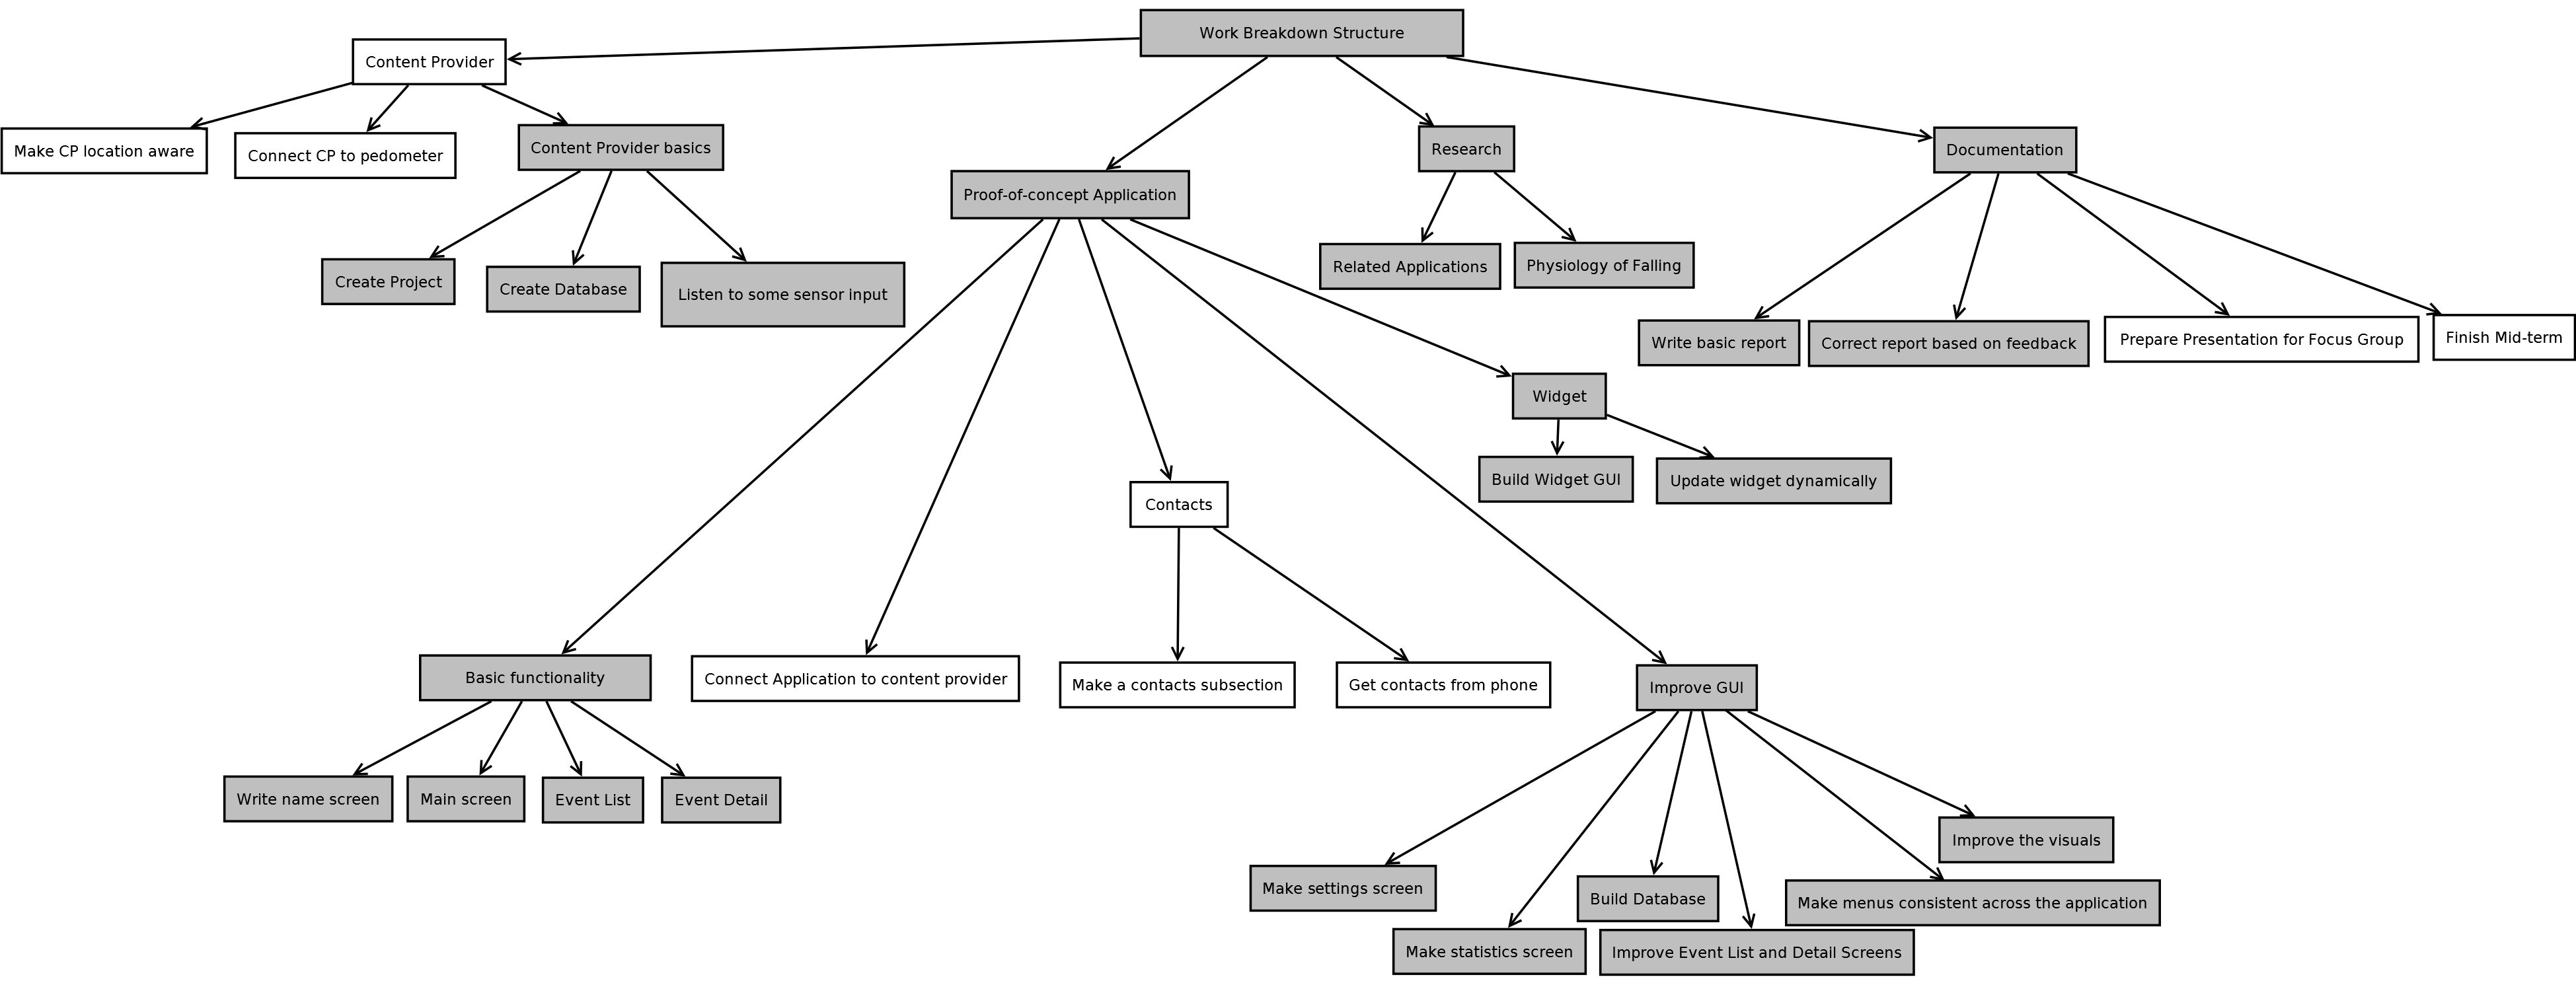
\includegraphics[width=1.45\textwidth , angle=270]{Res/WBS15313.png}
}
}

\caption{The current WBS}
\label{fig:WBS}
\end{figure}

\section{Development process}
\label{def:devProcess}

The customer favored the use of an iterative approach to the development process, where every sprint added a new layer of functionality, either to the application or the underlying model. Each sprint lasted for a period of 1-2 weeks, and the exact content was worked out in collaboration with the customer. Short term plans were favored over longer plans, due to the flexibility provided. While this made formulating definite goals for the final product difficult, the customer and the group were in agreement that due to the research intensive nature of the project, a high degree of flexibility was required. 

It was decided that the developers would have online meetings twice a week and an offline meeting once a week. 
The working hours were set to not less than 20 hours a week, but the developers were free to choose when to work themselves. This number was the expected workload for the course, and made a reasonable target for work per week. The meetings with the team was set to two times per week instead of once per day, so it could fit with the schedules of the team members. This was different from other agile methods like Scrum, but if was a necessary adaptation to fit meetings into the entire teams schedule. Updates were shared among the team members with email, Trello\footnote{See page \pageref{def:trello} for more info}, and it's learning as a replacement for daily meetings.
\subsection {How Tasks are assigned}
The group were using the working platform Trello from their website\footnote{https://trello.com/}, where the tasks are updated every week. Here tasks can be declared in a table of labeled with tasks "to do in future", "doing" and "done". This was done by the project manager and the document-organizer, see \ref{def:the group}, although all group members could ask to work on one part in particular. When the work was done, it was reported back to the board on trello, and a new task was assigned.  


\section{Software development}
\subsection{Agile software development}
Agile software development is a collection of software development methods. These methods were developed based on iterative and incremental software development. Agile development also cuts the working process into short periods of working time, which gives us the possibility to see the progress and act accordingly. Agile development focuses on evolutionary development, where the team can make a plan according to what has been done.  

\subsection{Iterative approach}
Iterative development simplified is a cycle of agreement, execution and assessment. Most engineering project using this approach also includes stages like requirements and design. The project using iterative development will enter several stages where these stages is repeated in a cycle formation. The cycle will usually contain a planning phase, which makes it relatively easy to react to a current problem, this can for instance be time spent and time left. The software is developed through several rounds with these cycles. 

\subsection{Extreme programming}
Extreme  programming is an agile software development methodology which favors improving of a software and quick responses. Extreme programming uses a cycle based programming system, but unlike the Iterative approach, it has a checkpoint after each stage, where the code is being released and new customer requirements is added.

\section{Group development method} 
At the beginning of the semester the group were given a task to develop an application system. At that time they did not have any idea on how the system as a whole would look like, but they were given small goals every sprint like developing specific parts of the application system. At this time they used a development method almost equal to Extreme programming, but took some concept from Scrum since they were more familiar with terms from Scrum like sprint. The method used gave possibilities for quick responses like editing the code to what the customer wanted or changing algorithms to more effective ones.

After Easter the group got a clearer vision of their final goal, and the development method were switched to Scrum development method. Clearer sprints were formed. Smaller task with estimated time usage were formed on Trello, as Trello were used more frequently than before. Tasks with similar working area were put together in a bigger assignment, but with the possibility to only do the one small task if they wanted to. After making the tasks the Group leader and the document-organizer could freely assign tasks to the rest of the group members, and tasks that had not been assigned were for those who would finish early with their work. This was done to organize the tasks to get a better overview for better planning.

\section{Meetings with customer and supervisor}
Weekly meetings with the customer took place every Friday, as explained above. Also, meetings with the supervisor were conducted every second week.

The meetings had several positive effects:
\begin{itemize}
\item The project stakeholders were kept up-to-date.
\item The progress of the project was predictable.
\item The developers got feedback before and after the tasks are done.
\item The project was split in small pieces of actionable and specific smaller tasks.
\item These smaller elements were discussed and considered before they were started.
\item Due to the smaller pieces of progress, mistakes were backtracked with a minimum of wasted work.
\item Customer got to participate in the development.
\item The group could take action when the supervisor or customer gave feedback on the results.
\end{itemize}


\section{Plans}

Nearing the end of every sprint, the customer and group agreed upon the content of the following sprint. This list has been placed in Figure \ref{tab:sprintList}, and provided a short summary of what was accomplished in a particular time-frame. 


\section{Team Roles and Organization}
\subsection{The group}
There was not much place for specific roles among the group, as it was a small group, and the project required that all the members were capable and willing to work at all the tasks. This makes a difference from development models with specific roles and tasks assigned. Roles that were set for the group were therefore mainly organizers, so that one person was to keep awareness of what work needed to be completed in a particular domain, and share it with the rest of the group:

\begin{description}

\item[Group Leader] Elias was made organizer, and got the responsibilities of reminding the group of what to do.
\item[Document-organizer] Johannes was tasked with organizing documentation and distributing the work of writing the report to the group. 
\end{description}
\subsection{Conflict handling}
There was no one-on-one conflicts, but some conflicts arose right after mid-term regarding work load and willingness to prioritize the prioritize. To try to solve this the group leader communicated the issues and its potential solutions via e-mail, with no further response. Some group members took the e-mail seriously and stepped up their work load, but on the other hand some ignored this wake up call completely and did not take any action. A meeting with the Supervisor was scheduled to try to get an idea to solve the situation, but was used for other purposes instead, because the group did not have an opportunity to discuss matters beforehand.
%TODO Add more here before delivering final report. 

\section{Comparison}
The development model used by the group was a form of agile development. Other well-known examples of agile methodologies are Scrum and Extreme Programming.
\section{Learning experiences from development and tool use}
Following are things that relate to project management and software development that the group learned during the project:
\begin{itemize}
 \item  It is important to ensure that documentation is done in a systematic fashion. In the beginning, a large amount of the reports and documentation that the group made for internal use, turned out to create more work and confusion later on. This was in part because it was not thought to be necessary at the time. Looking back, it seems like it would have been much more efficient to write reports well, and write them in LaTeX  while they were still new.
 \item Communication and what tools to use, was in flux for some time. Even when a few tools were settled on, the group still had problems with making sure all the members were on the same page regarding what needed to be done. 
 \item  Usage of tools which not all members were equally experienced with turned out to be problematic. This was because of misunderstanding and difficulties which could often be resolved by only one or two members, and slowed down the entire group. This might have been mitigated if all the members had a better understanding of the tools that were used. This could be accomplished by teaching sessions and group members being encouraged to seek a better understanding on their own.
 \end{itemize} 
  

